\documentclass[11pt]{report}

\usepackage{graphicx} % Required for inserting images
\usepackage{listings}
\usepackage{amsmath}

\title{SCNC2021 Report: An Analysis of Coalition Formation with Symmetric Agents}
\author{Eliz So (u7489812)}
\date{April 2025}

\begin{document}


\maketitle

\chapter{Introduction}
\paragraph{In competitive multi-agent environments, formation and dissolution of coalitions play a crucial role in shaping strategic outcomes. This research explores an algorithmic framework for evaluating coalition stability under a Cournot-style competition, where agents compete for limited resources such as market share, public attention, or user traffic. }
\paragraph{The algorithmic framework has two assumptions, that the agents in the game are indifferent to each other (the game is symmetric), and the linear and demand functions are linear. We implement a recursive, memorised function (sym\_split) that can systemically evaluate the utility of all possible coalition structures, and choose the best one out of it. }
\paragraph{The model is generalisable across different fields, including firm mergers in oligopolistic markets, political alliance in political advocacy coalitions, or even AI agent coordination. The model is a versatile tool for analysing cooperation and defection incentive in strategic settings.}
\paragraph{The primary objective of this research is to assess which coalition structures are stable, and explore the most efficient way to find the optimal coalition structure. }
\chapter{Literature Review}

\section{Theory of Agreements}

\paragraph{In Debraj Ray's A Game-Theoretic Perspective on Coalition Formation, the second chapter first provided definitions of a characteristic function and cooperative games. Specifically, it defined negotiations as a profile of actions that players would be willingly be signatories to, and characteristic function is a function that attaches each nonempty subset of players, or coalitions, to a set of possible payoff vector to each player a coalition \cite[Chapter 2]{ray2007ch2}. } \paragraph{Then, it introduces the two methodologies approaching to coalition formation in the book. The first method is to consider the entire process of coalition formation and writing binding agreements as a traditional noncooperative game, where a proposer attempting to form a coalition must make a proposal, and the members must accept or reject the proposal. The second approach is to consider coalitions as the fundamental units. This method means that the responses to proposals made are decided at a coalitional level instead of individual moves. Any objection will be studied as a coalitional block. }

\paragraph{Another important section that the algorithm may use is farsightedness. As the book states, whichever method you may use to consider coalition formation, the theory must consider the possibility that agents may look beyond the immediate consequence of their own actions. For instance, a firm (or person) might want to deviate from the coalition in the next step if a certain decision was made. That firm, or person, might consider how their utility would change before agreeing to make that decision. Furthermore, if a player or a group of player broke off their negotiation, they must be prepared for other players in their group to make further deviations, and that the larger group they have broken from might no longer be band together. }

\paragraph{The topic of this paper is related to the first example in the last section of chapter 2, Oligopoly. Showing that a 3-player Cournot oligopoly will end up with 3 firms banding up together, as any other coalition structure will mean there contains at least one firm that will deviate from the coalition, ending with a structure of individual firm coalitions. The utility of each firm in a grand coalition (banding together) is greater than deviating into 3 individual firms. Therefore, the firms will see that joining together in a coalition is their best solution. }

\paragraph{However, the given example does not state what happens when there are more firms, and the author has noted that being able to find the grand coalition will indeed form which can be obtained through characteristic function is entirely coincidental. As such, the rules to the dynamic programming algorithm will be referencing to the example to compute what the stable coalition structure would be with more than 3 firms.}

\section{Survey on Coalition Formation}

\paragraph{Moreover, a survey was read to understand better on the field of coalition formation. Rahwan et al. \cite{rahwan2015coalition} had discussed the coalition structure generation problem, and provided algorithms that helped to compute the optimal coalition structure that maximises social welfare. The survey first provided common definitions and notations in this field, then presented algorithm that computes an optimal coalition structure. Later, it discusses the coalition structure generation problem under various compact representations of the characteristic functions. After, the survey discusses games where a coalition is allowed to form under certain constraints. Finally, the survey discusses Partition Function Games. }
\paragraph{In this report, other than common definitions and notations, the relative topics are algorithms that searches for the optimal coalition structure, and Partition Function Games.}
\subsection{Common definitions and notations}
\paragraph{For starters, the coalition-formation process usually involves three main activities, forming a coalition structure, solving the optimisation problem of each coalition, and dividing the reward of each coalition among its members. The problem discussed in this report does contain the above, and will be further discussed under Section 3. }

\paragraph{The common notations stated in this survey will be notations that are used within this report for better readability. The definitions are as follows: }

\begin{itemize}
	\item \textbf{Coalition structure} over any coalition $C$ is a collection of coalitions, $CS = \{C_1, \dotso ,C_k\}$ such that $\cup CS =C$, and $C_i \cap C_j=\emptyset$ for any $i, j \in \{1, \dotso, k\} : i \neq j$. The coalition structures over C will then be denoted as $\prod^C$. 
	\item \textbf{Set of agents} in the game will be denoted as $A$.
	\item \textbf{Characteristic Function Games (CFGs)} are the games where the value of the coalition only depends on the identities of its members. 
	\item \textbf{Partition Function Games (PFGs)} are games where the value of the coalition depends on both the identities of its members and the way non-members are partitioned.
	\item \textbf{Search space} of the coalition structure generation problem is denoted as $\prod^A$, which is the space of all possible coalition structures over $A$.  
	\item \textbf{Coalition structure levels} $\prod_i^A$ represents all coalition structure containing exactly $i$ coalitions. 

\end{itemize}

\subsection{Coalition structure generation in PFGs}
\paragraph{The survey states that Lucas and Thrall \cite{lucas1963partition} who proposed Partition Function Games believe that externalities are a central notion of PFGs. Games with negative externalities ($PFG^-$) means that merging any two coalition will result in a worsen utility, and games with positive externalities ($PFG^+$) would benefit from two coalitions merging. Games with positive externalities may have overlapping or partially overlapping goals, so that coalitions can satisfy their own goals while satisfying some goals of other coalitions. }
\paragraph{The survey further states that a bound can be established with partial search, and that the value of all coalitions joined together would be larger than the coalition structures not joined together in a PFG+ setting. However, this only applies for social welfare, and not the individual utility value of each agent. In $PFG^+$ games, agents may leave their own coalition to maximise their own welfare, causing a worsen utility for the other coalition.}

\paragraph{In this report, the problem that will be stated later is closer to a game with positive externalities. The two coalitions that merged together would have a larger total utility than the two separated ($\frac{D}{(m+1)^2} \geq \frac{2D}{(m+2)^2}$), but the individual utility has more importance in the game presented. More will be explained in the Section 3.  }

\subsection{Algorithms and Searches}

\paragraph{The first algorithm the have presented is a dynamic programming (DP) algorithm, proposed by Yeh \cite{yeh1986dynamic}. The algorithm recursively looks through the value of a coalition, and compares with previous findings to find the value of an optimal partition of C. }
\paragraph{A weakness about this algorithm is that it is not an anytime exact algorithm. This means that running the algorithm longer may not necessarily improve the solution quality. Another is that the time complexity is still at $O(3^n)$. Rahwan et al. \cite{michalak2016hybrid} developed another version of DP, namely ODP, that can avoid evaluating many movements, and proved that they were using the least amount of movements. Yet, the time complexity is still at $O(3^n)$. Despite so, this optimised version avoids approximately two thirds of the operations compared to the original DP, which is less than $\omega (n^{n/2})$. A further description of the DP algorithm would be explained in 2.3. }
\paragraph{The survey then introduces anytime exact algorithms where the solution quality improves monotonically as computation time increases. The first algorithm introduced was developed by Rahwan et al. \cite{rahwan2009anytime}, an integer partition-based search called IP. It searches the space by the coalition size, then eliminates some search spaces when the maximum is smaller than the lower bound. Despite so, the time complexity of IP algorithm is still $O(n^n)$, and might even constructing every possible coalition structure in the worse case. Yet, if the situation contains a lot of coalition-value distributions, IP is significantly faster than ODP. }

\paragraph{Later on, an algorithm called ODP-IP was developed where it is an anytime dynamic programming-based search. As the name suggests, it combines both ODP and IP together. The operation of ODP is used to evaluate the movements through edges in the coalition structure graph, while IP deals with subspaces represented by integer partitions. In other words, the IP algorithm finds the coalitions that could maximise social welfare in that coalition structure. For a bound less than 5, the algorithm is able to run as fast as $O(\sqrt{n}2.09^n)$, faster than IP and DP. } 


\section{IP and DP}

\paragraph{Looking further into IP, DP, ODP and ODP-IP, Michalak et al.\cite{michalak2016hybrid} has written a paper explaining the algorithms with more details. }
\paragraph{Starting with the IP algorithm, it divides the space into different coalition structures, so that we can compute the upper and lower bounds on the value of the best coalition structure in each subspace. Then, $Max_s$ and $Avg_s$ is the maximum and average values of the coalitions in $C_s^A$ respectively. Further, let I(i) be the multiplicity of i in I, where $I\in T^n$. $T^n$ is the set of all integer partitions of n. Then, }
\[\frac{\sum_{CS\in \prod_I^A} V(CS)}{|\prod_I^A|}=\sum_{i\in I}(I(i)Avg_i) \]
\paragraph{Since the value of the best coalition structure in the subspace is the average value, we can then let the lower bound of the value of the best coalition structure in $\prod^A_I:LB_I=\sum_{i\in I}(I(i)Avg_i)$. The upper bound can be found by replacing $Avg_i$ with $Max_i$. The algorithm then computes an upper bound $\text{UB*}= \max_{i\in I}\text{UB}_I$ and an lower bound $\text{LB*} = \max_{i\in I}\text{LB}_I$ on the value of an optimal coalition structure CS*. The upper bound UB* helps us to bound the quality of CS**, which is the best coalition structure found by the algorithm at a given point in time. The lower bound LB* helps us to identify subspaces that has no potential to provide the optimal coalition structure. Subspaces $\prod_I^A$ with $\text{UB}_I<\text{LB*}$ are pruned from the search space. }

\paragraph{When searching a subspace, the algorithm uses a depth-first manner. It iterates over the coalitions in $C_{i_1}^A$ and every coalition $C_1 \in C_{i_1}^A$ encounters, it iterates over the coalitions in $C_{i_2}$ that do not overlap with $C_1$. This means that every coalition structure might be examined more than once. However, the search can be sped up by using a branch-and-bound technique at every depth $d < k$. where $d$ is the number of coalitions, where $k$ is the number of relevant coalitions. Before iterating through the coalitions, the algorithm checks if }
\[\sum_{j=1}^dv(C_j)+\sum_{j=d+1}^kMax_{i_j}<V(CS^{**})\]
\paragraph{If the inequality holds, every coalition structure containing $C_1, \dotso, C_d$ can be skipped because the value cannot be greater than the value of the best coalition structure found by the algorithm so far. }

\paragraph{Next, the DP algorithm follows the below theorem strictly.  }
\paragraph{Given a coalition $C \subseteq A $, let $f(c)$ be the value of an optimal coalition structure over C (i.e. $f(C)=\max_{CS\in\prod^C} V(CS)$).  Then, }
\[f(C) = \begin{cases}
	v(C) &\textbf{if }|C|=1 \\
	\max\{v(C), \max_{\{C', C''\}\in\prod^C}f(C')+f(C'')\} & \textbf{otherwise}
\end{cases}\]

\paragraph{It should be noted that DP requires storing a total of $2^{n+1}$ values, which is f(C) and t(C), a variable that provides an indication of the optimal partition of C. Since the input to the problem already contains $2^n$ values already, they just assume that there will be $O(2^n)$ available space. }

\paragraph{The DP algorithm can be optimised, also known as ODP. What DP does initially is to first evaluate all the movements in the graph, store the most beneficial movements, and move upwards in the graph. We can see that for every coalition structure CS with $|CS|>2$, there are multiple paths start from the bottom node of the graph that end with the node that contains CS. Therefore, we can remove some movements that are redundant, so that we can still reach CS without repeating. Michalak et al. proved that the number of movements $|M^*|$ is equal to the number of coalition structure in levels 2 and 3 of the coalition structure graph. Formally, }
\[|M^*|=|\prod_2^A|+|\prod_3^A|\]

\paragraph{Michalak et al. \cite{michalak2016hybrid} suggested the ODP-IP Algorithm. It contains an integer partition graph where every node represents an integer partition. Within each node, the IP algorithm searches for the optimal coalition structure. Within the graph, the ODP algorithm searches for the integer partition with the greatest value. }
\paragraph{Finally, to improve the efficiency, IP can be modified to search multiple subspaces simultaneously and to avoid repeating certain operations. It states that for each coalition structure, the algorithm shall find the best partition in later levels that contains the original coalitions, and find the best coalition structure out of all of them. If one partition multiple coalitions, more subspaces can be searched simultaneously.}

\paragraph{The ODP-IP algorithm inspired the algorithm created in this research project. Given that the firms are all symmetric, a DP algorithm was used to go through an integer partition graph. However, IP algorithm is not needed for each node as symmetric means all coalition structure under that integer partition node will produce the same utility. }
\section{Computing Best Response}
\paragraph{Looking into Elkind et al.'s \cite{elkind2021bestresponse} method of finding best response, it had requirements such as it must be a Tullock contests with convex costs. The cost function also had to be twice differentiable, zero cost for no-participation, increasing and weakly convex. Therefore, another method of computing the best response was used. Bravo et al.'s \cite{bravo2018bandit} method focuses on games with finite number of payers, and that are a concave game, such as the Cournot competition. The method uses regularised no-regret learning. It uses mirror descent to generate a new feasible point $x^+$ by taking a mirror step from the starting point $x$ along the direction of an "approximate gradient" $y$.}
\paragraph{If players are able to obtain gradient information by first-order oracle, which is a feedback mechanism that provides an estimate individual payoff gradient, then the best response can be calculated along with regularised no-regret learning. The first-order feedback does not need perfect information in this case. }

\paragraph{If players do not have access to first-order oracle, they can use bandit payoffs which derives an individual payoff gradient by the actual payoffs at each stage. In this research, players know the demand and cost equations, as they are all symmetric to each other. Therefore, they can estimate their individual payoff gradient without neding to derive it. In other words, they have access to the first-order oracle, and do not need to use bandit payoffs. }
\chapter{Problem Statement}
\paragraph{In this report, the aim is to understand more about different coalition structure, explicitly, what are the stable coalitions in a game with $n$ firms. Referring to Ray \cite[Chapter 2]{ray2007ch2}, three firms with same linear demand function and cost function would always be in one same coalition to maximise their profit. However, what happens with a game with other number of firms? And is there a pattern to the stable coalition structures?}

\paragraph{The game this report analyses is an extension of Antoine Cournot's theory of competition \cite{cournot1838} , Cournot oligopoly. The theory describes how firms in an imperfectly competitive market will compete by choosing the quantity of output independently and simultaneously. Instead of only making a choice in the quantity of output, the game allows the firms to collude to be in a coalition. The game first assumes that all firms are in a grand coalition. Then, the firms have the choice to leave the coalition and choose the quantity of output.}

\paragraph{In this game, the rules are simple. Agents in a coalition have two choices, to stay or leave. For simplicity, the algorithm will consider the utility of the agent at zeroth index.  leaving the coalition $C$ is defined as a group of agents $C'$, where $|C'| \leq \frac{|C|}2$ forms a new coalition. To consider whether a firm or coalition wants to stay or leave a coalition, they will see if they have an incentive to leave. The incentive is decided as would their utility after leaving be larger than their current utility. }
\paragraph{All agents of this game will have a demand function $P(Q)$, cost function $c(q)$, and a utility function $u(Q, q)$ based on the total quantity $Q$ and individual quantity $q$. For ease, the analysis provided will have a linear demand and cost function. However, the production code does provide an option for different types of demand function, including power, exponential, and log.}


\paragraph{From the survey, it states that the three main activities in coalition-formation process. Firstly, the algorithm finds the best response, which will be the Nash Equilibrium in this case. This solves the optimisation problem of each coalition. Next, in terms of dividing the reward of each coalition among its members, there are a few solutions. The Shapley-Shubix power index is a measurement that is normalised between 0 and 1 \cite{shapley1954power} , where 0 means that the agent has no effect on the outcome, and 1 means the agent determines the outcome. Suppose that there are $n+1$ members, each member can vote once, and each member has $k_i$ votes. Then, each member has a power index of $\frac{k_i}{n+1}$. Now consider where $m$ firms are symmetric in a coalition, where they all decide to produce the same quantity. As such, their power index of each firm would be as follows:  }
\[\frac{q_1}{m+1}=\frac{q_2}{m+1}=\dots=\frac{q_m}{m+1}\]
\paragraph{Thus, no firms outweighs the other in terms of the Shapley-Shubik power index. Hence, the reward, also known as the utility of the coalition would be distributed evenly amongst the firms of the coalition. }
\paragraph{Lastly, with forming a coalition structure, this report uses a version of DP that is tailored to the problem. The algorithm used for this problem has modified to consider the utility function of one person instead of the entire coalition. Given the game is symmetric, same utilities will appear the same for the same coalition structure. Therefore, IP algorithm is not used here.}
\paragraph{Ultimately, there shall be an explanation on the algorithms used and their result. Moreover, an example of application in real life will be provided.}


\chapter{The algorithm}
\section{Finding the Best Response}
\subsection{Demand function}
\paragraph{The demand function $P(Q)$ is set to be linear for this problem statement where $Q$ is the total quantity and }
\[P(Q)=A+BQ\]
\subsection{Cost function}
\paragraph{For this problem statement, the cost function is to be set as }
\[c_i(q_i) = dq_i\]
\subsection{Utility function}
\paragraph{The utility function $u_i$ is to find the profit of each agent. The utility function is defined as follows, }
\[u_i = P(Q)-c_i(q_i)\]
\paragraph{Where $P$ is the demand function, $Q$ is the total quantity, $c_i$ is the cost function of each agent $i$ and $q_i$ is the quantity for each agent. }

\subsection{Nash Equilibrium} 
\paragraph{The definition of Nash Equilibrium is the set of strategies such that no player can unilaterally deviate from their strategy to get a higher payoff, given the strategies of all other players \cite{nash1950equilibrium}. Formally, we can let}

\begin{itemize}
	\item $A$ as the set of players
	\item $S_i$ as the set of strategies available to player
	\item $S$ as all strategy profiles
	\item $u_i$ as the payoff function for each player $i$
\end{itemize}

\paragraph{Then, $s^*\in S$ is a Nash Equilibrium of a strategic game if and only if $\forall i \in A$ and $\forall s_i \in S_i$, }
\[u_i(s_i^*, s_{-i}^* \geq u_i(s_i, s_{-i}^*)\]


\subsection{Best Response }
\paragraph{Best response is a strategy that gives the highest possible payoff for a player, given the strategies chosen by other players \cite{nash1951noncooperative}. Formally, the definition is }
\[BR_i(s_{-i}) = \{s_i \in S_i | u_i(s_i, s_{-i}) \geq u_i(s_i', s_{-i}) \forall s'_{i} \in S_i \}  \]

\paragraph{The best response in this problem statement can then be considered as }
\[BR_i(Q-q_i) = \max_{q_i' \geq 0}\{P(Q-q_i+q_i')q_i'-c_i(q_i')\}\]
\paragraph{Therefore, we can find the best response of each firm by finding the differentiated equation of the utility function. The maximum value should be when the differntiated value is 0. And thus, we can find $q_i'$ that way. }

\[\frac{du_i}{dq_i}=\frac{\delta}{\delta q_i}P(Q)-\frac{\delta}{\delta q_i}c_i(q_i') = 0\]

\subsection{Theorem 1}
\paragraph{By using Taylor's series, $f(x+h)$ and $f(x-h)$ can be expressed as the following equations \cite{rudin1967principles}}
\[f(x+h)=f(x) + hf'(x) + \frac{h^2}{2}f''(x) + \dots\]
\[f(x-h) = f(x) -hf'(x)+\frac{h^2}{2}f''(x)+\dots \]

\paragraph{Therefore, it can be rewritten as}
\[f(x+h)-f(x-h)=2(hf'(x)+\frac{h^3}{6}f'''(x)+\dots)\]
\[\frac{f(x+h)-f(x-h)}{2h}=f'(x) +\frac{h^2}{6}f'''(x)+\dots\]

\paragraph{If $h=1e^{-10}\approx0$, }

\[\frac{f(x+h)-f(x-h)}{2h}\approx f'(x)\]

\subsection{Finding the new quantity}

\paragraph{The rest of the calculation part has referenced Bravo et al. \cite{bravo2018bandit} theory on finding the Nash Equilibrium in concave n-person games. Using gradient descent, we use a small step size to slowly get closer to the actual quantity. The small step size $k$ is calculated by $\frac{0.05}{\sqrt{t+1}}$. Each new value of the quantity would be as follow}
\[q_{i_{new}}=q_{i_{old}}+k \frac{du_i}{dq_i}\]
\paragraph{If $q_{i_{new}}$ is smaller than 0, $q_{i_{new}}$ would be set as 0.}

\subsection{Initial Quantity}
\paragraph{Firstly, the quantity should be initialised according to the demand function of the market. Given when the demand function $P(Q)$ is linear,}
\[P(Q) = A -B\times Q\]
\paragraph{If the total quantity  of the firms $Q$ is larger than or equal to $A$, then $P(Q)$ will be less than or equal to 0, implying the firms would have a negative profit. Therefore, it should be ensured that $Q<A$.}
\paragraph{Recall that}
\[Q=\sum_{i=1}^nq_i\]
\paragraph{Assuming all firms should be looked equally initially, the initial quantity for each firm should satisfy}
\[q_i\leq\frac{A}{Bn}\]
\paragraph{The optimal quantity for higher utility increases as more coalition appears, as $P(Q)$ is a linear equation with a negative slope (i.e. $B < 0$). Hence, the initial quantity would be set as follows, }
\[q_i^{init}=\frac{A}{Bmn}\]
\newpage 
\subsection{Putting the algorithm together}

\paragraph{The best response function shall first find the utility for each coalition, then split the reward to firms amongst the coalition. The algorithm is written as follow: }

\

\begin{lstlisting}

def BR(state, demand, cost)
    
    MAX_ITER = 10000
    
    //Finding the initial quantity for each coalition. 
    qs_coals = [A/(B*m)] * m 
    
    qs = [A/(B*n*m)] * n 

    for t in 0...MAX_ITER:
        Q = sum(qs)
        
        prev_coals = qs_coals.copy()
        curr_coals = qs_coals.copy()

        for i in 0...m:
        
            // find the new value of q
            q = calculation(Q, demand, cost, prev_coals) 
            curr_coals[i] = q
            
        for i in 0...m:
            
            if new_utility > old_utility:
                qs_coals = curr_coals[i]
                assign qs_coals to qs 
       
       if change of qs < 1e-8:
           break
   utils = [P(Q)*qs[firm]-cost(qs[firm]) for firm in range(n)]        
   
   return qs, utils


\end{lstlisting}

\section{Finding the Stable Coalition}
\paragraph{In finding the stable coalition, since the firms are all symmetric, the algorithm can search through the coalition structures instead of individual coalition combination. With this method, we can minimise the search space from $O(Bell(n))$ (where Bell() is the bell numbers) \cite{bell1934} to $O(\exp(\sqrt{n}))$ \cite{andrews1998partition}. The figures 4.1 and 4.2 show the differences between searching the stability of individual coalition combinations instead of coalition structure. }

\begin{figure}[htbp]
	\centering
	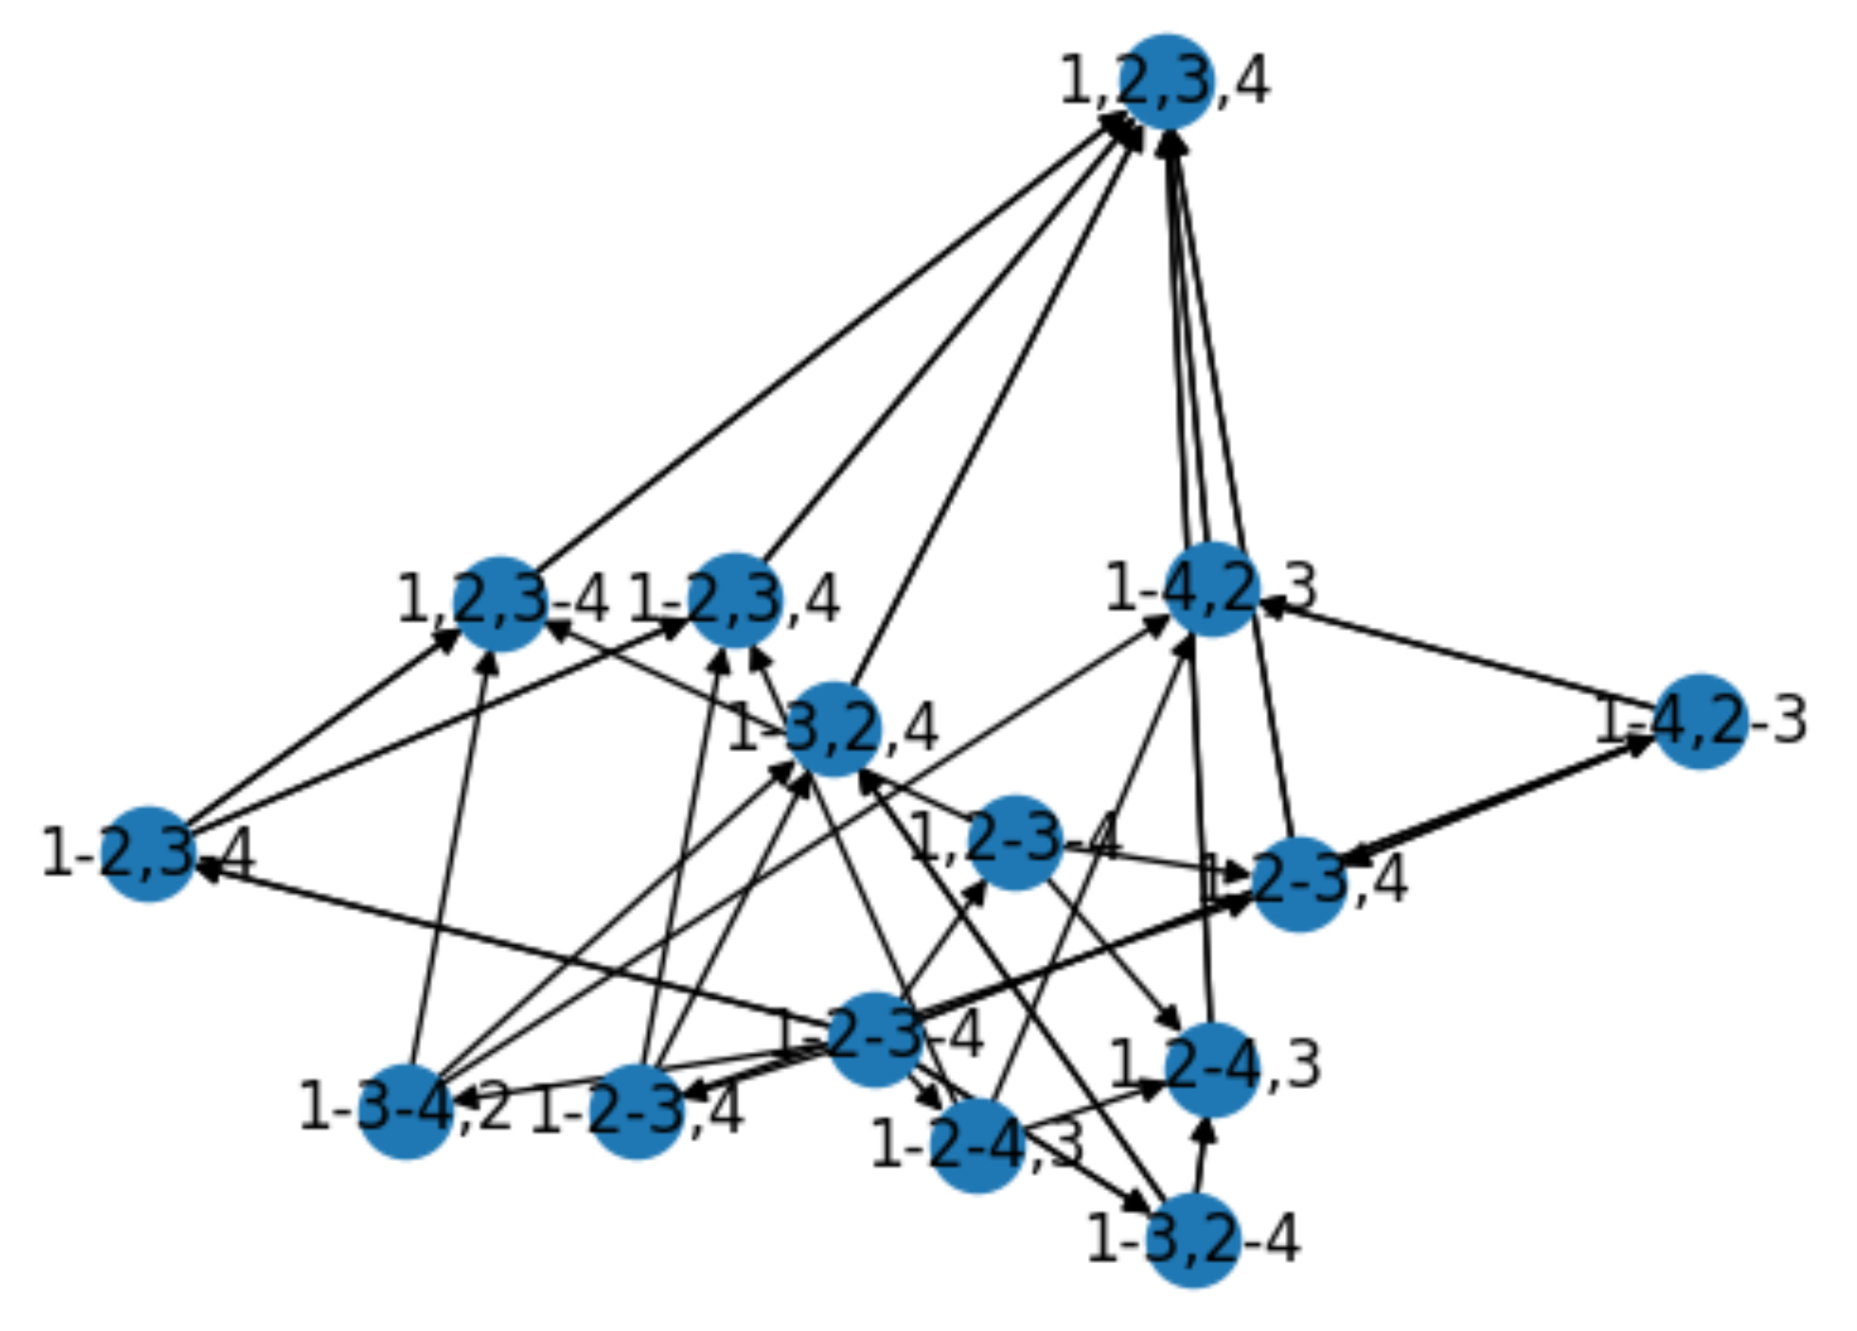
\includegraphics[width=0.5\textwidth]{images/nonsym4.jpeg}
	\caption{individual coalition combinations}
\end{figure}

\begin{figure}[htbp]
	\centering
	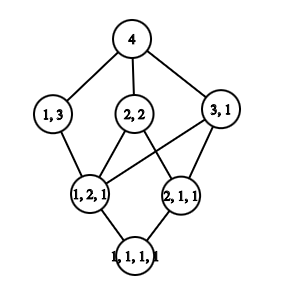
\includegraphics[width=0.5\textwidth]{images/sym4.png}
	\caption{coalition structure}	
\end{figure}


\subsection{Notations}
\paragraph{In this section, the notations are as follows. A tuple shows the coalition structure, displaying how many firms in one coalition. For instance, (1, 3, 2) would mean there is one firm in a coalition,  three firms in the second coalition, and 2 firms in the last coalition. Furthermore, the coalition in the zeroth index is the firm we are considering. The rest of the coalitions are sorted in reverse order to search in the dictionary later. It should be noted that tuples can be hashed in Python, which can assist in searching the keys in dictionary.} 

\subsection{DP algorithm }
\paragraph{The DP algorithm depends directly on the following: }
\[
DP_i(s) = 
\begin{cases}

u_i(q_i, Q) &\text{if no one has incentive to deviate } \\
f(k_{1_i}, k_{2_i}) &\text{else}
\end{cases}
\]
where 
\[
\begin{align}
	k_{1_i} &= \max_{s'\in S_i} DP(s', i) \\
	k_{2_i} &= \min_{s'\notin S_i} DP(s', i) \\ 
	f(k_{1_i}, k_{2_i}) &= \max(k_{1_i}, k_{2_i}) 
\end{align}
\] 

\paragraph{The DP algorithm states that if no agents have incentive to deviate, their utility value shall stay the same. Otherwise, $k_{1_i}$ computes the maximum utility when the agent decides to leave by itself, or with other agents. $k_{i_2}$ computes the minimum utility when other agents decide to leave, finding the worst case scenario, as the agent cannot anticipate nor control what other agents will do.} 
\paragraph{Lastly, $f(k_{1_i}, k_{2_i})$ is the function representing an agent deciding whether to stay or leave the firm. In this case, we will assume that the agent would like to maximise their utility, and thus choosing the maximum out of the two. }

\paragraph{The python code shall be seen in the production code as the sym\_split function. }
\section{Parallel Processing}
\paragraph{To make the algorithm more efficient, parallel processing can be implemented to search more spaces in the same time. Once the space had been searched, the algorithm does not search it again. Instead, the value is saved into a dictionary. It is recommended that the first layer of search is done in parallel, as there can be limitations to distributing too many tasks to limited CPUs. While memory lock can be used, it will slow down the algorithm. Thus, it is not recommended to use memory lock. }

\section{Complexity}

\paragraph{Firstly, the time complexity of the best response function depends on how many coalitions does the current state has. Therefore, the time complexity is $O(m)$ where m is the number of coalitions. }

\paragraph{Assuming the algorithm attempts to exhaustively search through all the coalition structure, it would take $O(B(n))$ where $B(n)$ is the Bell number \cite{bell1934}. Bell numbers grow faster than exponential, making it a super-exponential time complexity. This implies that it would be infeasible to use even for moderate values of n. However, we reduced the search space by only searching through the integer partitions through dynamic programming. }
 
\paragraph{Without parallelisation, the proof for it's time complexity is as follow: }

\paragraph{Firstly, the number of unique states for each run is the same as the partition of n, which is $\exp^{\pi\sqrt{2n/3}}=O(\exp(\sqrt{n}))$\cite{andrews1998partition}. As such, we know that the total number of sym\_split() calls made is at most $O(\exp(\sqrt{n}))$, as it has a memorisation check to skip states that have already been computed. }
\paragraph{Next, it computes the utility of the current coalition structure. It attempts to lookup at the dictionary, otherwise calls best\_response() which costs $O(m)$. Then it attempts to split from the coalition first, which calls up to $n/2$ recursive calls. And attempts to split coalition from the rest, which is at most $\frac{n-1}2$. Thus, the total overhead should be $O(m+n)$. Since $m \leq n$ always, this can be simplified to $O(n)$. }

\paragraph{Finally, by multiplying the number of unique states by the per-state cost, we have }
\[T(n) = O(\text{no. of states}) \times O(\text{work per state}) 
= O(n\exp(\sqrt{n}))
\]

\paragraph{a quasi-polynomial time complexity, which is expensive but still manageable for $n\leq30$. }

\paragraph{As for the space complexity, the dictionary that saves all the destination stores each unique state as the key. Therefore, there should be number of integer partitions of n total firms $O(\exp({\sqrt{n}}))$. As each entry stores the coalition state and the final utility vector, which is of length n, the space required for the destination dictionary is $O(n\exp(\sqrt{n}))$. }

\paragraph{For the utility dictionary, it stores the utility of coalition of size k in a partition of length m. The possible values of m goes from 1 to n, and for each, the possible value of k goes from 1 to n to. While the worst-case size is $O(n^2)$, it is much often smaller in practice. }

\paragraph{Lastly, the call stack space is the maximum depth of recursion, which is when coalition halves at each level. Thus, it is $O(\log n)$. By adding them up together, we would have $O(n\exp(\sqrt{n}) + n^2 + \log n) = O(n\exp(\sqrt{n})) $. This also implies that the space complexity is mostly dependent on the destination dictionary. }

\paragraph{With parallelisation, the time complexity reduces as the number of workers you have. Given that if you have $p$ processors, the runtime should be }
\[\frac{T(n)}{p}=\frac{n\exp(\sqrt{n})}{p}\]

\paragraph{However, since multiprocessing allows each worker to get its own copy of the dictionaries and task inputs, there will be $p$ copies of all data during active execution. Therefore, the total space with $p$ workers is: }
\[O(p\cdot n\exp(\sqrt{n}))\]
\paragraph{In which, the memory pressure can become significant if n is large and p is high.  }
\chapter{Results}
\section{Example}
\paragraph{In Ray\cite{ray2007coalitionformation}, the example showed what happens with 3 firms. The firms ended up in a grand coalition as it benefits them more than separating apart. However, for situations with more firms, grand coalition may not be the solution. In fact, there could be more than 1 stable solutions for larger number of firms. }
\paragraph{For example, a coalition structure of (2, 2, 2, 1, 1) can be a stable for 8 firms. In the algorithm, since it starts splitting from the grand coalition, it finds the first stable coalition structure that can maximise the first firm's profit according to 5.2.3.}
\paragraph{In an example of 10 firms, the algorithm outputs (1, 7, 2). Figure 5.1 can assist in explaining the given output. The column states how many firms are in one coalition, and the row shows how many coalitions are there in the solution. The cells with green colour is what the utility would be for the solution. Cells in red are the utilities that would be smaller than splitting into 10 firms. Cells in grey are the utilities that are not possible for this number of firm. If the coalition structure contains any combination with red cells, it implies there is definitely a better option for all the firms in that coalition, where everyone is in a coalition of 1. }


\begin{figure}
	\centering
	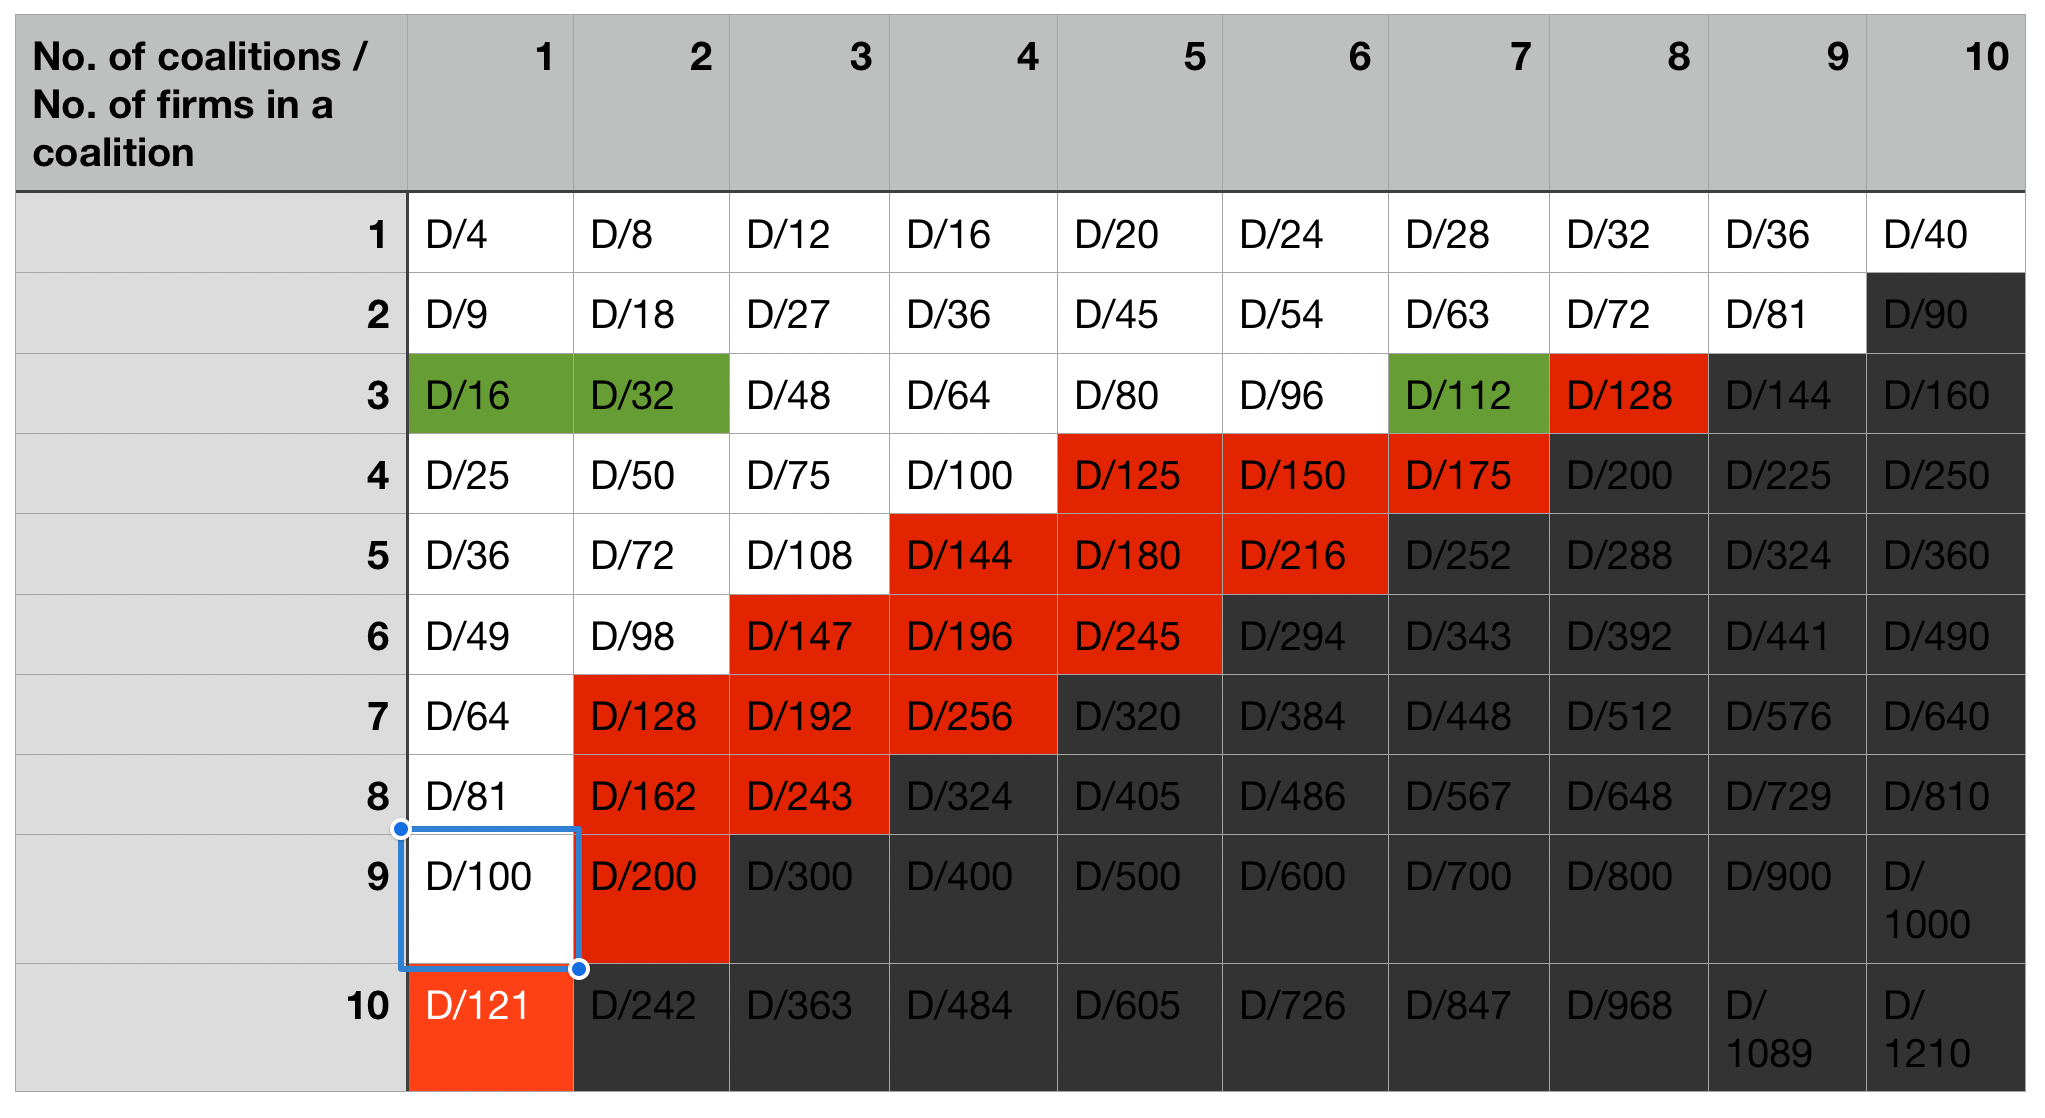
\includegraphics[width=0.7\textwidth]{images/coalition.jpeg}
	\caption{coalition utility for 10 firms at each level}
\end{figure}

\paragraph{Note that in the coming analysis, firm one no longer has the option to leave the coalition as the coalition only contains itself. Starting from the stable coalition, an analysis can be made to check if there are any firms who want to deviate according to the algorithm.}

\paragraph{Firstly, we can consider if any of the 7 firms would want to deviate. If one or two firm deviates, it is certain that more firms will deviate from the coalition, as it lands in one of the red cells. If three firms deviate, forming (1, 4, 3, 2), we have to follow through the algorithm to find the minimum utility for the 0th indexed firm. To ensure that the coalition structures are still landing on the white colour cells, 2 firms from the 1st indexed coalition can leave first, forming (1, 3, 2, 2, 2). Then, 1 firm from the 1st indexed coalition can leave again, forming (1, 2, 1, 2, 2, 2). This coalition structure has a utility of D/49 and D/98, where $D=\frac{(A-c)^2}{b}$\cite{ray2007coalitionformation} for all firms, in which D/98 is smaller than the utility when the 7 firms are grouped together. Knowing the worst case scenario, the 7 firms would not deviate in this situation.}
\paragraph{Now consider the coalition with 2 firms. When a firm leaves from the coalition, it forms the coalition structure (1, 7, 1, 1), leaving the coalition with 6 firms to land on a red cell in the figure. Thus, a deviation must happen in this case. Again, to ensure that the 0th indexed firm is getting the smallest utility, the coalition structure becomes (1, 4, 3, 1, 1), then (1, 3, 2, 2, 1, 1), and finally (1, 2, 2, 2, 1, 1, 1) is the only stable coalition structure before everyone is in a coalition of 1. Since it also leads to a utility of D/49 and D/98, which both of them are smaller than D/48, the firms in that coalition would not be willing to deviate from their coalition. 
}
\paragraph{Therefore, no firms would be willing to deviate from their coalitions at (1, 7, 2). }

\paragraph{While there might contain other coalition structures that are stable, it might not be the minimum of the zeroth index firm, or that the algorithm had searched this coalition structure after (1, 7, 2).}

\section{Analysis}
\paragraph{The default values used in the production code are: }

\[P(Q)=100-2Q\]
\[c_i(q_i)=10q_i\]

\paragraph{The table below shows the stable coalition structure that the algorithm generates for $n$ firms for the default values from the production code}
\begin{center}
\begin{tabular}{c c }
  	number of firms & coalition structure \\ 
  	1 & (1)\\ 
  	2 & (2)\\
  	3 & (3)\\ 
  	4 & (4)\\
  	5 & (1, 2, 2)\\
  	6 & (1, 3, 2)\\
  	7 & (2, 5)\\
  	8 & (1, 5, 2)\\
  	9 & (1, 6, 2)\\
  	10 & (1, 7, 2)\\
  	11 & (2, 9)\\
  	n = [12, 50] & (1, n-3, 2)\\ 
\end{tabular}
\end{center}

\paragraph{From the table, it can be seen that firms would only stay in the grand coalition when $n \leq 4$. Otherwise, firms prefer to split into different coalitions. However, it seems that when $5 \leq n \leq  11$ there is no consistent pattern to the stable coalition. The smallest coalition switches between 1 to 2 firms. Yet, when $12 \leq n \leq 50$, the coalition structure has a consistent pattern of (1, n-3, 2). While there might be other coalition structure that are stable for those number of firms, we can at least expect that a grand coalition does not happen, and that it may be possible that duopoly or monopoly exists in the market.}

\paragraph{This result may be important to policymakers when they are legislating new laws regarding a certain business sector, or how agents decide to collaborate or not, as they might need to expect deviations from others too. This will be further explained in the next section.}



\chapter{Application In Real Life}

\section{Political Advocacy Coalitions}
\paragraph{The first case is that several political advocacy groups are trying to gain public attention through different media, such as media coverage, social media engagement, or public support. As they push their message, the space becomes more crowded. Therefore, the attention becomes scarce and competitive. }
\paragraph{We can first treat the public attention as market demand, and each political advocacy coalition is like a firm in a Cournot competition. We can also let total message volume from all coalitions be $Q$, and how effectively each unit gets noticed is }
\[P(Q)=a-bQ\]
\paragraph{Where }
\begin{itemize}
	\item a = 100, which is the maximum attention one coalition is broadcasting
	\item b=2, each additional message reduces marginal attention
\end{itemize}
\paragraph{As for the cost, each coalition would have to pay a certain cost to craft and deliver messages, such as advertisements, having events, or putting posts up. We can quantify it by putting a cost per unit message (e.g. $c=10$). }
\[C_i(q_i)=c\cdot q_i \]

\paragraph{Now, imagine there are five coalitions of advocacy groups: }
\begin{itemize}
	\item Environmental group (EG)
	\item Indigenous rights group (IR)
	\item Anti-poverty coalition (AP)
	\item Housing justice network (HJ)
	\item Migrant rights coalition (MR)
\end{itemize}
\paragraph{Initially the five coalitions can be working together to get a quantity of 4.5, and a utility of 202.50 each. However, this is not the most efficient way of getting their messages across. }
\paragraph{Let assume that we are working for EG, and we have been asked to evaluate whether we should continue working with other groups. }
\paragraph{From the table in the previous section, we can see that five firms ends up with a coalition structure of (1, 2, 2). It implies that EG should work solo, as their utility becomes 253.12 eventually. Even if they do not end up with (1, 2, 2) and stop at (1, 4), EG will still have a utility of 450.}

\section{Merging APIs}
\paragraph{Consider 6 AI agents are trying to provide API agents to developers and companies, where each agent competes for limited developer attention. These AI agents can either operate independently or form coalitions, such as co-branded access, or shared APIs, etc. }
\paragraph{It should be noted that we assume that these AI agents provide the same service, and are indifferent in price too. }

\paragraph{Let the demand function P be the average willingness to pay per API call, and Q be the total API traffic from all agents. The cost would be the cost per API call, including cloud computing, bandwidth, etc.}

\paragraph{If the agents are currently working independently, each agent has the utility of 82.65. Two agents may consider about merging together. }

\paragraph{If we call the sym\_split function, where firms = 2, and rest = (1, 1, 1, 1), we can see that it is not a stable coalition structure, that it would split back into 6 independent agents. This is because that merging together does not increase the utility of the two individuals, and decreases it to 56.25.}

\paragraph{Now if two agents decide to merge together, and three other agents are merging together, the last agent can see if the coalition structure is stable. Again, if we call sym\_split where firms = 1, and rest = (3, 2), the last agent can expect that the certain coalition structure should last. If any firms deviate, they will result in a lower utility at 82.65. }


\chapter{Conclusion}
\paragraph{This research demonstrates the power of recursive, memorised algorithms in modelling coalition dynamics under Cournot competition. By applying the sym\_split function to linear Cournot settings, we can identify the equilibrium coalition structures that maximises agent utility while accounting for potential deviations. }
\paragraph{While the model derived from the economic theory, its applications can extend to political and AI contexts, where agents coordinate, compete, and adapt in response to shifting payoffs. The framework can provide both theoretical insight and practical tools for exploring how agents align or defect in shared environments.  }

\paragraph{In the future, the analysis can consider other types of demand and cost function, such as, power, exponential, logarithm. Also, other economic theories can be considered. For instance, an agent can be an "evil git". This implies that if they see another agent deviating and decreases their utility, their aim will no longer only be maximising their own utility, but to minimise the agent harming their utility.}

\bibliographystyle{plain}
\bibliography{subfiles/references} 

\end{document}

